\documentclass{sigchi}

% Use this command to override the default ACM copyright statement
% (e.g. for preprints).  Consult the conference website for the
% camera-ready copyright statement.


%% EXAMPLE BEGIN -- HOW TO OVERRIDE THE DEFAULT COPYRIGHT STRIP -- (July 22, 2013 - Paul Baumann)
% \toappear{Permission to make digital or hard copies of all or part of this work for personal or classroom use is      granted without fee provided that copies are not made or distributed for profit or commercial advantage and that copies bear this notice and the full citation on the first page. Copyrights for components of this work owned by others than ACM must be honored. Abstracting with credit is permitted. To copy otherwise, or republish, to post on servers or to redistribute to lists, requires prior specific permission and/or a fee. Request permissions from permissions@acm.org. \\
% {\emph{CHI'14}}, April 26--May 1, 2014, Toronto, Canada. \\
% Copyright \copyright~2014 ACM ISBN/14/04...\$15.00. \\
% DOI string from ACM form confirmation}
%% EXAMPLE END -- HOW TO OVERRIDE THE DEFAULT COPYRIGHT STRIP -- (July 22, 2013 - Paul Baumann)


% Arabic page numbers for submission.  Remove this line to eliminate
% page numbers for the camera ready copy 

%\pagenumbering{arabic}

% Load basic packages
\usepackage{balance}  % to better equalize the last page
\usepackage{graphics} % for EPS, load graphicx instead 
%\usepackage[T1]{fontenc}
\usepackage{txfonts}
\usepackage{times}    % comment if you want LaTeX's default font
\usepackage[pdftex]{hyperref}
% \usepackage{url}      % llt: nicely formatted URLs
\usepackage{color}
\usepackage{textcomp}
\usepackage{booktabs}
\usepackage{ccicons}
\usepackage{todonotes}

% llt: Define a global style for URLs, rather that the default one
\makeatletter
\def\url@leostyle{%
  \@ifundefined{selectfont}{\def\UrlFont{\sf}}{\def\UrlFont{\small\bf\ttfamily}}}
\makeatother
\urlstyle{leo}

% To make various LaTeX processors do the right thing with page size.
\def\pprw{8.5in}
\def\pprh{11in}
\special{papersize=\pprw,\pprh}
\setlength{\paperwidth}{\pprw}
\setlength{\paperheight}{\pprh}
\setlength{\pdfpagewidth}{\pprw}
\setlength{\pdfpageheight}{\pprh}

% Make sure hyperref comes last of your loaded packages, to give it a
% fighting chance of not being over-written, since its job is to
% redefine many LaTeX commands.
\definecolor{linkColor}{RGB}{6,125,233}
\hypersetup{%
  pdftitle={SIGCHI Conference Proceedings Format},
  pdfauthor={LaTeX},
  pdfkeywords={SIGCHI, proceedings, archival format},
  bookmarksnumbered,
  pdfstartview={FitH},
  colorlinks,
  citecolor=black,
  filecolor=black,
  linkcolor=black,
  urlcolor=linkColor,
  breaklinks=true,
}

% create a shortcut to typeset table headings
% \newcommand\tabhead[1]{\small\textbf{#1}}

% End of preamble. Here it comes the document.
\begin{document}

\title{BehaviorSim Model Builder: Lessons Learned Designing for JiTAI Developers}

% \numberofauthors{5}
% \author{%
%   \alignauthor{Tylar Murray \\
%     \affaddr{University of South Florida}\\% Department of Electrical Engineering}\\
%     \affaddr{Tampa, USA}\\
%     \email{tylarmurray@mail.usf.edu}\\
%     }
%   \alignauthor{Eric Hekler\\
%     \affaddr{Arizona State University}\\% School of Nutrition and Health Promotion}\\
%     \affaddr{Phoenix, USA}\\
%     %\email{e-mail address}
%     }
%   \alignauthor{Donna Spruijt-Metz \\
%     \affaddr{University of Southern California}\\% Center for Economic and Social Research}\\
%     \affaddr{ Los Angeles, USA}\\
%     %\email{e-mail address}\\
%     }
%   \alignauthor{Daniel E. Rivera \\
%     \affaddr{Arizona State University}\\% Control Systems Engineering Laboratory}\\
%     \affaddr{Tempe, USA}\\
%     %\email{e-mail address}\\
%     }
%   \alignauthor{Andrew Raij \\
%     \affaddr{University of Central Florida}\\% Institute for Simulation and Training}\\
%     \affaddr{Orlando, USA}\\
%     %\email{e-mail address}\\
%     }
% }

\maketitle

\begin{abstract}
In this paper we present design considerations relevant to the development of software for behavioral scientists creating Just-in-Time-Adaptive-Interventions (JiTAIs). 
Our findings are based off of a user-survey of behavioral scientists, expert-panel reviews, and user-experience interviews performed in development of the BehaviorSim model-building tool. 
Lessons learned through iterations of this tool, a JiTAI developer user persona, and guidelines for those targeting behavioral scientists as a user group are highlighted. 
\end{abstract}

%TODO:
\keywords{Authors' choice; of terms; separated; by semi\-colons;
  commas, within terms only; this section is required.}

%TODO:
\category{H.5.m.}{Information Interfaces and Presentation
  (e.g. HCI)}{Miscellaneous} \category{See
  \url{http://acm.org/about/class/1998/} for the full list of ACM
  classifiers. This section is required.}{}{}

\section{Introduction}
% JiTAIs?
% * what is the problem with current behavioral science research methods?
With the increasing prevalence of wearable technologies and personal health data, behavioral researchers are becoming increasingly overwhelmed with data.
Researchers have seen the potential for optimizing a behavioral intervention to suit not only the user \cite{beck2010challenges}, but also the context \cite{brailsford2010towards, collins2004}. 
Just-in-Time Adaptive Interventions (JiTAIs) promise to provide the optimal nudge at the optimal time to aid users looking to change their behavior \cite{nahum2014}.
Imagine, for example, an anti-stress app which knows not to interrupt work meetings, but also knows when to play a favorite song to help relieve stress on the drive home.
Or consider a smoking cessation app that knows precisely when and where craving is most likely, and distracts with a game before the desire to smoke is noticeable.

The impending wave of context-aware\cite{schilit1994context}, affective computing\cite{picard2000affective} applications seems to be the holy grail of behavior change, but researchers are finding that our models of human behavior are not capable of supporting this level of interaction.
Existing  models of behavior do not offer the granularity and specificity needed for these applications\cite{riley2011health}.
Currently, psychological models of human behavior act as a guide for behavioral scientists looking to predict behavior, but are rarely computational in nature - making direct application to adaptive systems impossible.
Methods for creating computational models of human behavior are not well defined, but some early concepts have been published \cite{rivera2013systems}.

% TODO: ADD THESE?:
% b/c of ubiquitous mobile & sensor tech
%    dynamical systems are good way to model at this level

\section{Methodology}
% SBM Survey 
A preliminary survey was given to a group of behavioral scientists in order to gauge the general perceptions and opinions on the development of behavioral models to support JiTAIs.
In this survey we focused on a few key elements of the model building process to greatly simplify and shorten the modeling exercise.
A contextual and behavioral outcome based on physical activity were given, and users efforts were focused on defining the inner workings of the human system within these constraints.
We also asked participants to complete survey items about the barriers facing modeling and simulation in behavioral science.
Approximately 50 surveys were distributed following presentations on behavioral modeling and simulation at the 35th Annual Conference of the Society of Behavioral Medicine. 
Out of these 50, only 12 surveys were returned.
In general, users had trouble with even the simplified modeling exercise.
Most did not stray far from the given example, and others provided very different solutions which could not be reconsiled with the ``engineer's view'' of the problem.
In the survey questions participants reported that the mathematics and programming concepts required for developing simulatable models were overwhelming, and nearly all participants expressed a desire for increased collaboration between disciplines and a need for software tools to help them apply and validate these methods.


% behaviorSim model-builder v1
Using findings from the user study we developed a proof-of-concept software to aid behavioral researchers with the task of building a computational behavioral model. 
The software - called the behaviorSim Model-Builder (see figure \ref{model-builder-v1}) - took a step-wise approach towards the model-building process.
First users are asked to list environmental inflows, internal state variables, and behavioral outflows of the model explicitly during the ``think'' stage.
Next, users are prompted to define the connections between nodes, ``draw''ing the model's structure.
Lastly, users are required to ``specify'' the functional relationships at each node's inflow(s).
% TODO: include graphic which shows context/state/behavioral as mentioned in P above?

\begin{figure}[!t]
  \centering
  1 
  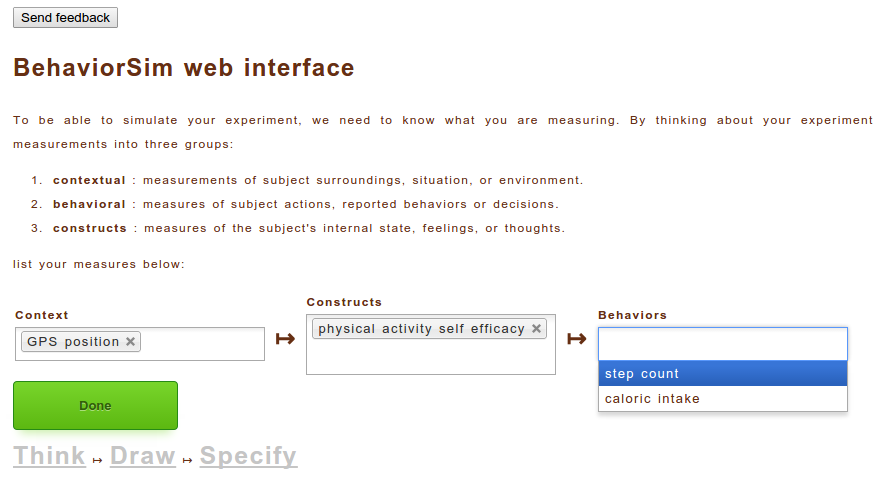
\includegraphics[width=0.9\columnwidth]{img/v1-think}
  \rule{\columnwidth}{0.4pt}
  2
  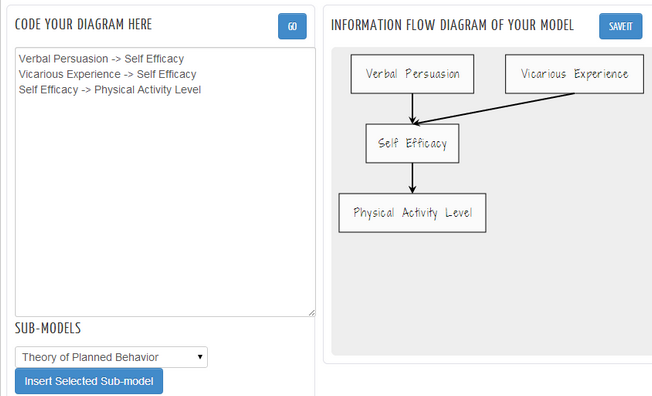
\includegraphics[width=0.9\columnwidth]{img/v1-draw}
  \rule{\columnwidth}{0.4pt}
  3
  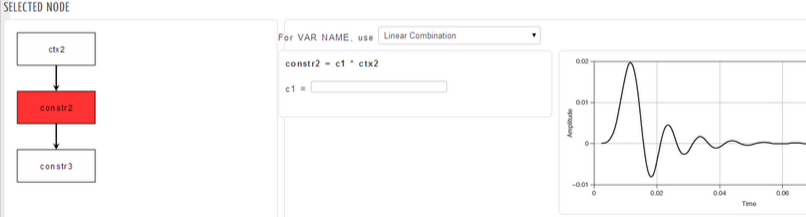
\includegraphics[width=0.9\columnwidth]{img/v1-specify}  
  \caption{behaviorSim Model Builder v0.1.x implemented three separate stages of model building as separate pages: 1) think, 2) draw, 3) specify.}
  \label{model-builder-v1}
\end{figure}

The model builder was reviewed by an expert panel of 2 behavioral scientists and 1 human-computer interaction expert. 
Though the steps in the outlined model development process seemed appropriate, it quickly became obvious that a step-wise design is not optimal.
Users who are forced to explore the process step-by-step have difficulty understanding how earlier choices related to later results, and feel constrained by previous choices rather than backtracking to revise the model.
This design does not allow for quick iteration on models, and requires the user to maintain a great deal of planning information internally.
% Though the information flow diagram employed in this version worked well to convey information about the model to the users, the graph was also assumed to be interactive - participants made attempts to modify the graph by clicking, and attempted to select nodes in the specification stage by clicking on them.
Our review concluded that a less constrained approach to the stages of the modeling process was needed, and a greater focus on the graphical model could greatly improve user experience.

% \subsection{behaviorSim Model-Building Tutorial v1}
After reviewing v1 of the behaviorSim Model Builder tool, a tutorial was designed to help bridge the knowledge gap for new modelers looking to use the tool.
In theory, the tutorial would help users see the bigger picture before diving into the stepwise process.
The tutorial was implemented as a walk-through of a simple example model's internals.
The tutorial introduced a hybridized information-flow and time-series graph, wherein each node of the graph contains a time-series spanning a common time-frame, and a user interface for adjusting model parameters and updating time-series values instantaneously (see figure \ref{model-builder-tutorial}).
This real-time parameter tweaking enables some degree of reconciliation with expectations of the data.

The same expert panel review process was as used for the evaluation of the tutorial. 
Through this evaluation it became clear that - although we had taken a step in the right direction, an even more explicit definition of terms was needed in order to clarify persistent disciplinary differences.
Reviewers also wanted better explanation of model input parameters and of the functional definition of the system.
They were not content with the hard-coded environmental inputs and wanted to be able to define how the contextual inflows changed over time.
Though the hybrid graph was found helpful in conveying the connection between path diagram nodes and time series, the shared time-axis was not obvious, and reviewers expressed a need for more explicit x and y axes as well as a better explanation as to what ``10 units of self efficacy'' actually means.
The time-series view was found to be both critical for the development of an accurate model, and valuable as pedagogical exercise for users trying to internalize model formulations.
 
\begin{figure}[!t]
  \centering
  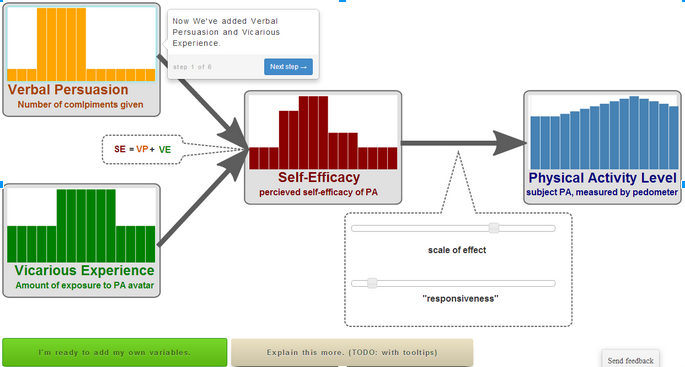
\includegraphics[width=0.9\columnwidth]{img/v1-flow}  
  \caption{behaviorSim Model Builder tutorial attempted to merge time-series and information-flow graph representations.}
  \label{model-builder-tutorial}
\end{figure}

% \subsection{behaviorSim Model-Building Tool v2}
Using what we had learned so far, the behaviorSim Model Building tool was re-designed and re-assessed.
In this version all steps of the modeling process (think, draw, specifiy) are unified into a single-page application, allowing users to see how choices influence the model in real-time, and thus can iterate on their design more easily (see figure \ref{model-builder-v2}).
The time-series charts popular in the tutorial were added as a ``mini-simulation'', to help users to visualize how variables change over time according to their model formulation.
To address the terminology gap which plagued v1, a set of tool-tips were added which revealed detailed definitions for key terms used in the user interface.
% In addition, the second version incorporates findings from the v1 tutorial, adding a ``miniature simulation'' to the application to allow for ``reconciliation and ``play''.
In this version of the tool, users declare constructs and define the structure of their model simultaneously by specifying on the connections using a simple Diagram Specification Language (DSL). 
In contrast to version 1, where the construct type had to be input by the user, the type of each node (contextual input, internal state, or behavioral measure) is inferred from the number of inflows and outflows.

The ``miniature simulation'' concept allows users to specify hypothetical contexts in which to explore the model dynamics, without the need to specify the full model.
Users can specify environmental inflows for the simulation, choosing from adjustable presets (square wave, step function, random walk, or constant value).
Selecting nodes on the graph by clicking, users can traverse the graph in any order.
Time-series plots of inflows as well as the resulting outflow at each node are provided using the miniature simulation model instance.
Internal state and behavioral measure nodes are specified similarly to environmental inflows through customization of function presets such as ``linear combination'' and ``fluid flow analogy''\cite{martin2014dynamical}.

\begin{figure}[!t]
  \centering
  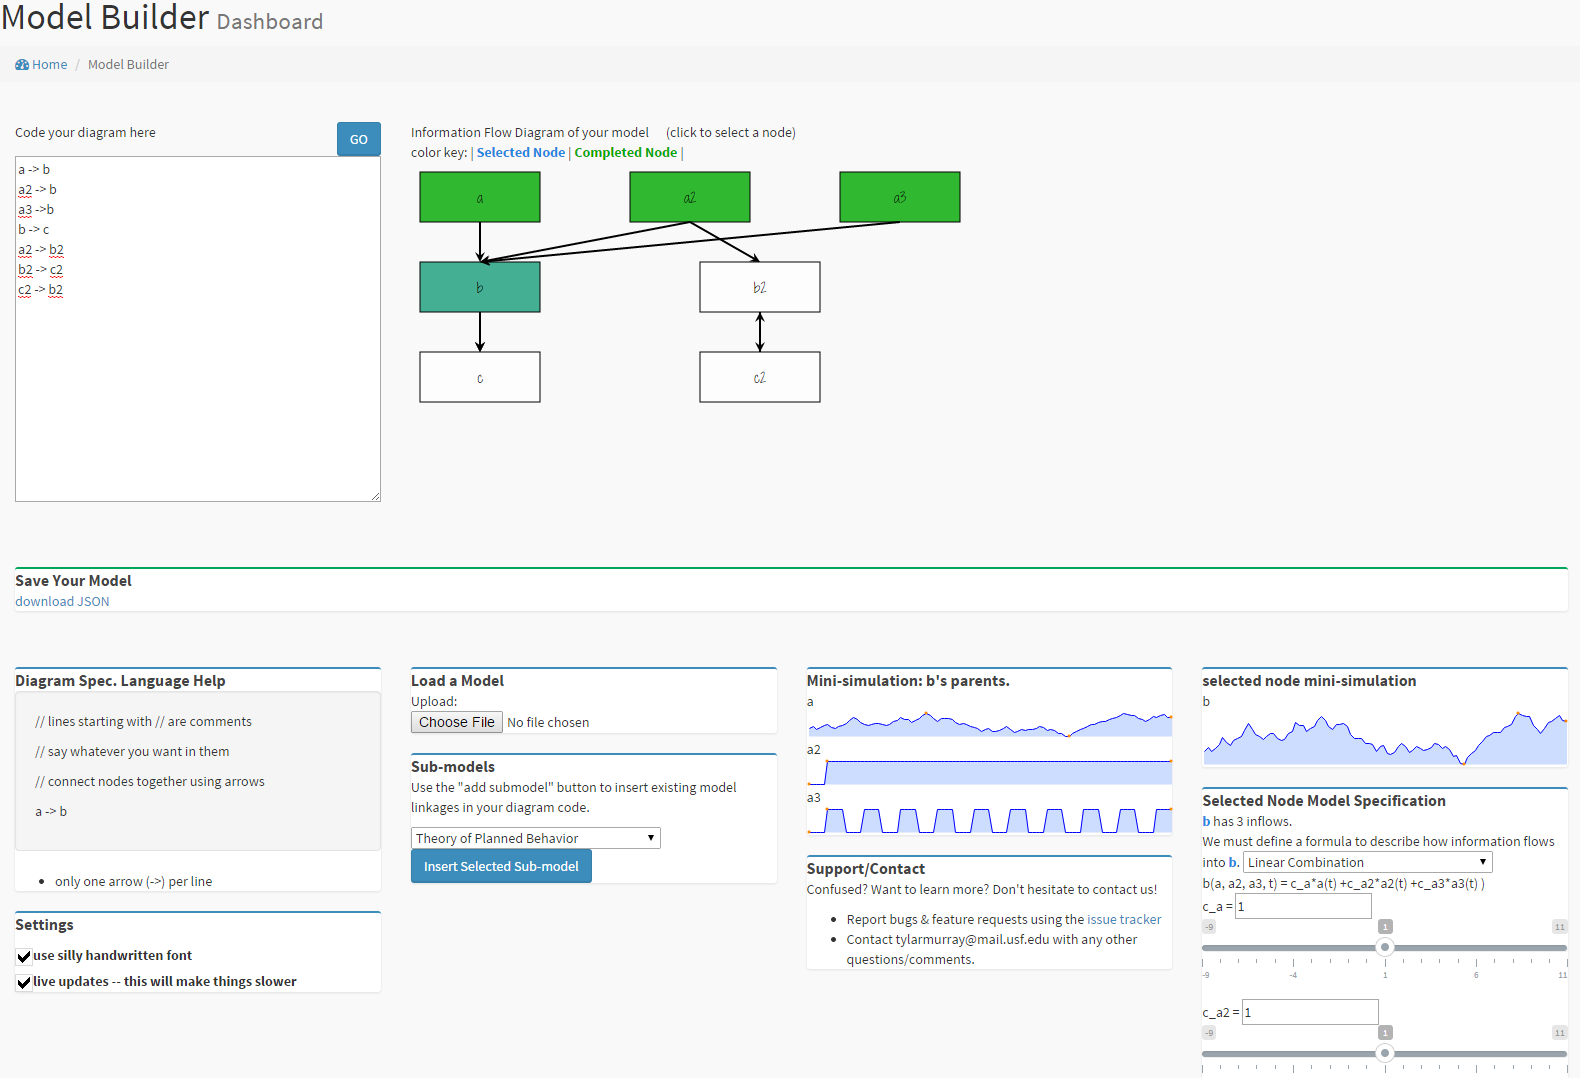
\includegraphics[width=0.9\columnwidth]{img/v2}  
  \caption{behaviorSim Model Builder v2 combines elements into a single view.}
  \label{model-builder-v2}
\end{figure}

This version was used as part of a structured exercise and interview outlining the design of a JiTAI to combat obesity.
The content of this exercise was based on recent work done to define the JiTAI design use-case \cite{nahum2015building}.
Preliminary findings from this exercise completed with 4 behavioral researchers highlight both the strengths and the remaining weaknesses of our design.
A think-aloud protocol was used while the software was in use, and the concluding interview gives insight to what users find most valuable, least valuable, and most in need of improvement.

Though the single-page design of version two did seem to allow for increased ability to iteratively explore models, reviewers now found the user interface somewhat overwhelming.
% Upon starting the review, users often felt unsure where to start.
Furthermore the connection between the information flow graphic and the related UI elements below was not always obvious.
% Reviewers did identify the relationship after some exploration, however. 
Additionally, the common user interface for specifying constructs regardless of node type broke down the distinction between environmental inflows, state variables, and behavioral outputs. This lead to to some confusion when specifying the various types of nodes.
Further contributing to this problem, the meaning of the mini-simulation was not always clear to reviewers, though the inclusion of time-series graphs was found helpful for understanding the model functions and their parameters once explained.
Nodes on the graph were made to change color when the specification process was complete, but reviews revealed that this was not a significant enough indicator of node ``completeness'', so that the user is sometimes unsure when they should feel free to move to the next node.
% Inclusion of a ``next node'' button which appears upon node specification completion may be all that is needed to help alleviate this issue.

\section{Results}
Our findings above reveal specific weaknesses in our design, and through analysis of these findings we present the following design guidelines for any software made to empower JiTAI developers.
Firstly we outline a rough JiTAI developer user persona based on our assessment of the general population of researchers in behavioral intervention design.
Next, we propose user stories and use-case details for the task of JiTAI design and evaluation.
Lastly, we provide some generic design guidelines which we have found to be particularly relevant in this design space.
% Please don't hate me too much for calling it a design ``space''

\subsection{JiTAI Developer User Persona}
% outline a rough JiTAI developer user persona based on our assessment of the general population of researchers in behavioral intervention design.
In general, JiTAI developers are behavioral researchers who see the powerful potential of ubiquitous computing for high-frequency data collection, automated analysis, intervention deployment, and personalization.
It is important to note that the research questions of a JiTAI researcher often differ significantly from the questions a behavioral scientist might typically have.
% “old” way vs “new” way not valid
The ``traditional'' way of modeling for behavior change relies primarily on statistical data analysis techniques to find relationships between variables on large time-scales.
In contrast, the JiTAI researcher needs to translate these relationships into a small-time-scale model which provides guidance regarding which interventions are most effective at which specific time(s).
% research questions have changed
Research questions focusing on the detailed dynamics of behavioral change are becoming increasingly prevalent as mobile behavioral health research continues to grow, and these are the kind of research questions that are of most interest to a JiTAI developer.

% modeling turns story into equations
The JiTAI developer wants to turn a patient story into a set of equations that can be handled by an automated system.
However, JiTAI developers typically do not have the level of familiarity with modeling systems to define abstract psychological models mathematically.
Furthermore, the psychological models commonly used are ill-specified at the (small) timescales of greatest interest, and often do not fit commonly used modeling paradigms - making mathematical definition a unique challenge for even a systems engineer.

The JiTAI developer wants to deploy and test a hypothesis by comparing model predictions to experimental data.
Statistical analysis techniques typically used to assess control vs experimental group differences are much less applicable to this problem, but the JiTAI developer often has little experience applying goodness-of-fit metrics.

% NOTE: actually, I covered this a bit in the above section.
% \subsection{What do JiTAI Developers Want?}
% propose user stories and use-case details for the task of JiTAI design and  evaluation
% First and foremost JiTAI developers want to 

\subsection{Guidelines for JiTAI Developer Softwar}
% provide some generic design guidelines which we have found to be particularly relevant in this design space

\subsubsection{Promote Expertise Development}
% information-seeking to aid learning of new concepts
%     access new terminologies/concepts for describing/defining model
%         existing model explorer to inspire/inform
%         existing data explorer to inspire/inform
The science of JiTAIs is young, and - as our user persona shows - behavioral scientists looking to work with JiTAIs are likely to run into many new concepts.
The potential complexity of a JiTAI system, however, may benefit from the use of advanced and specialized graphs, charts, and user interfaces. 
Thus, the needs of a novice user versus an expert user may be very different.
Because of this, software to support JiTAI development needs to promote the development of expertise in both the system and the relevant concepts through steady changes to the user interface \cite{cockburn2014supporting}.
In our case, a guided walkthrough of the software interface was sufficient, but we believe that a more graded approach would be more effective. 

\subsubsection{Enable Quick Iterations}
%    ease-of-iteration to allow quick iteration
%        changes easy and quick
%        allow comparison between before/after change
%        preserve modeling history, encourage undo/redo
The value of iterating on a design spans many domains, and is very applicable to the development of JiTAIs. 
Through our studies we have found that the development of even a simple JiTAI requires many iterations.
Thus, a software to aid in JiTAI development must allow for quick and easy modification, comparison, and reversion.
A comparison between the usage of our multi-staged model builder versus the single-page application showed a dramatic increase in the number of model iterations along with reported user comprehension.
Iterations on the model tended to follow a moment of realization or the learning of a new concept.
Thus, allowing for quick iterations allows for the user to more quickly apply newly gained expertise, yielding a better model and increased understanding.

%     model-probing tools (time-series) to test that model fits mental model
%        simulations
%        data-reconciliation
To encourage iteration in the JiTAI development process, assessment tools available part-way through the process - like our mini-simulation time-series - allow users to test their mental model of the system against its digital representation.
Allowing for more assessment points throughout JiTAI development allows users to identify problems early so they may iterate before the error cascades further through the process.

\subsubsection{High-Level Visuals to De-internalize Models}
%    model state-storage & reference visuals to de-internalize mental model
%        ease memory load
%        externalize model computations
Traditionally, psychological models of human behavior are meant to be guidelines for thinking about human behavior.
When using these models, the researcher must internalize the model and think through the subjects' state.
With JiTAI models, internalization of the full system becomes impossible due to the rise in specificity and complexity.
Thus, JiTAI development software must provide visualizations of the system to ease cognitive load on the user.
Focus plus context displays \cite{baudisch2001focus} can be used to allow users to delve into the specifics of a portion of the model without losing the larger context. 
In the behaviorSim Model Builder, we focus on the specification of a single variable at a time, and highlight this variable’s context in an information-flow path diagram of the model structure.
This dual-viewing-area approach works well for comparing variable details, but the use of a zoomable interface such as is employed in some flow-based programming \cite{morrison2010flow} tools may be more intuitive.
%    related design guides
%        FBP

\subsubsection{Adaptive Interface}
%    customizable interface & concept/model/data display tailored to research area
Though our JiTAI developer persona yields widely applicable general user stories, it is also important to recognize the diversity of the JiTAI developer user group.
JiTAIs are applicable to any area of behavior change; just a few popular proposed JiTAI applications are: management of eating behaviors, physical activity, smoking cessation, drug abuse, PTSD, and stress.
Within each of these many application domains, are a myriad of behavioral theories - further adding to the diversity of the user group.
Each of these sub-user-groups may have slightly different needs as they develop a JiTAI.
Furthermore, a JiTAI development software requires a standardized behavioral model or JiTAI format, and with that comes the opportunity to enable easy sharing and searching of JiTAI designs.
Thus, personalization of the software interface - to adapt the process or to offer relevant information\cite{kay2012creating} - can greatly improve user experience in this domain.

\section{conclusion}
TODO!

\section{Acknowledgments}

TODO!

% Balancing columns in a ref list is a bit of a pain because you
% either use a hack like flushend or balance, or manually insert
% a column break.  http://www.tex.ac.uk/cgi-bin/texfaq2html?label=balance
% multicols doesn't work because we're already in two-column mode,
% and flushend isn't awesome, so I choose balance.  See this
% for more info: http://cs.brown.edu/system/software/latex/doc/balance.pdf
%
% Note that in a perfect world balance wants to be in the first
% column of the last page.
%
% If balance doesn't work for you, you can remove that and
% hard-code a column break into the bbl file right before you
% submit:
%
% http://stackoverflow.com/questions/2149854/how-to-manually-equalize-columns-
% in-an-ieee-paper-if-using-bibtex
%
% Or, just remove \balance and give up on balancing the last page.
%
\balance{}

% REFERENCES FORMAT
% References must be the same font size as other body text.
\bibliographystyle{SIGCHI-Reference-Format}
\bibliography{sample}

\end{document}

%%% Local Variables:
%%% mode: latex
%%% TeX-master: t
%%% End:
